\documentclass{article}
\usepackage[utf8]{inputenc}
\usepackage{listings}
\usepackage{color}
\usepackage{graphicx}

\title{Laporan Database Trigger dan View}
\author{Ilham Dwi Prasetyo Nugroho}

\begin{document}
\maketitle
\section{Trigger, View, Table}
\subsection{Trigger}
\par Trigger merupakan kumpulan script yang berhubungan dengan table, view ataupun skema yang dijalankan secara otomatis ketika terdapat event yang dijalankan
\subsection{View}
\par View adalah objek di dalam database yang berisi kumpulan kolom yang dihasilkan dari Perintah select. Dengan kata lain yang lebih sederhana, view adalah object yang menyimpan hasil query, baik dari satu tabel atau lebih, didalam database view juga sering dinamakan sebagai “tabel virtual” , karena view sebenarnya tidak memiliki data. Data yang ditampilkan oleh sebuah view diambil dari tabel-tabel aktual yang disertakan dalam SELECT.
\subsection{Table}
\par Tabel adalah merupakan kumpulan dari beberapa record dan juga field
\section{Cara Pembuatan Trigger dan view di APEX online}
\subsection{pembuatan table}
\par pertama buka aplikasi oracle online dengan memasukkan workspace,username, dan password
\begin{figure}[h]
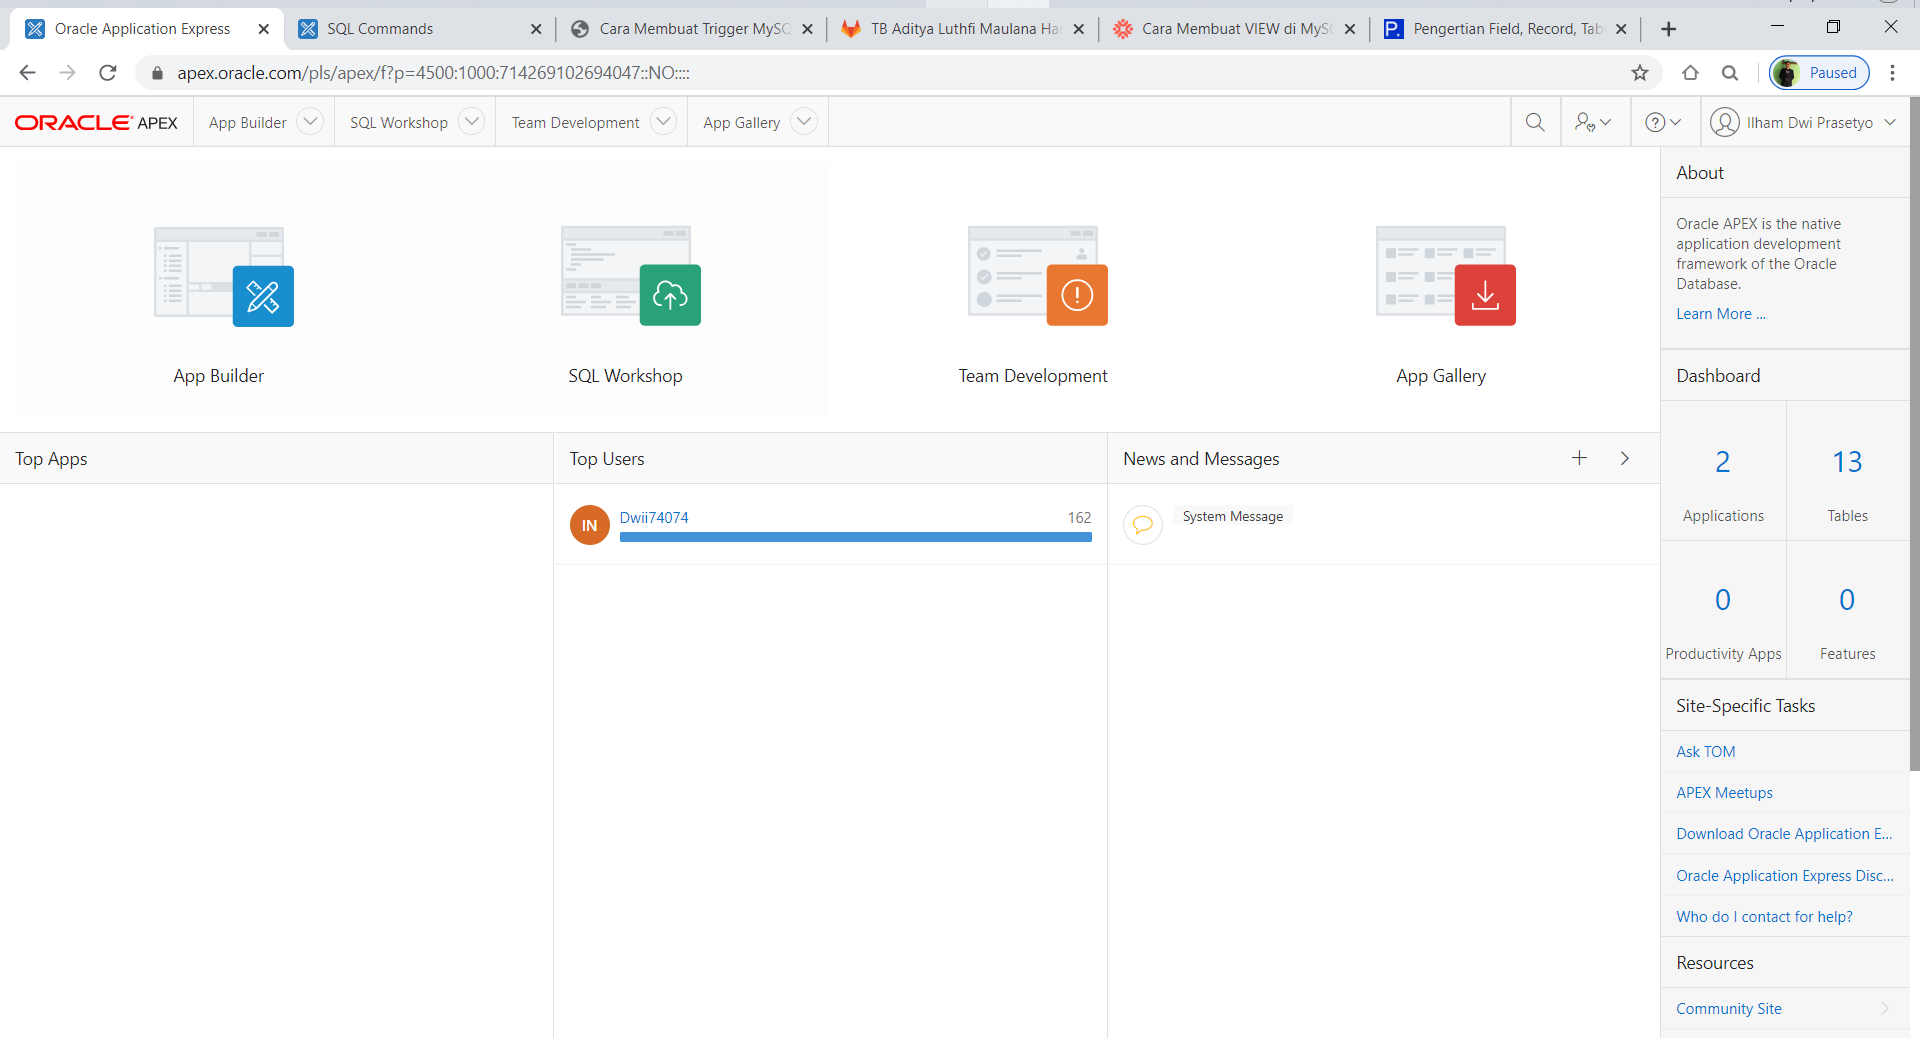
\includegraphics[scale=0.3]{img/1.PNG}
\end{figure}
\\
\\
\\
\\
\\
\\
\\
\\
\\
\par lalu masuk kedalam sql workshop
\begin{figure}[h]
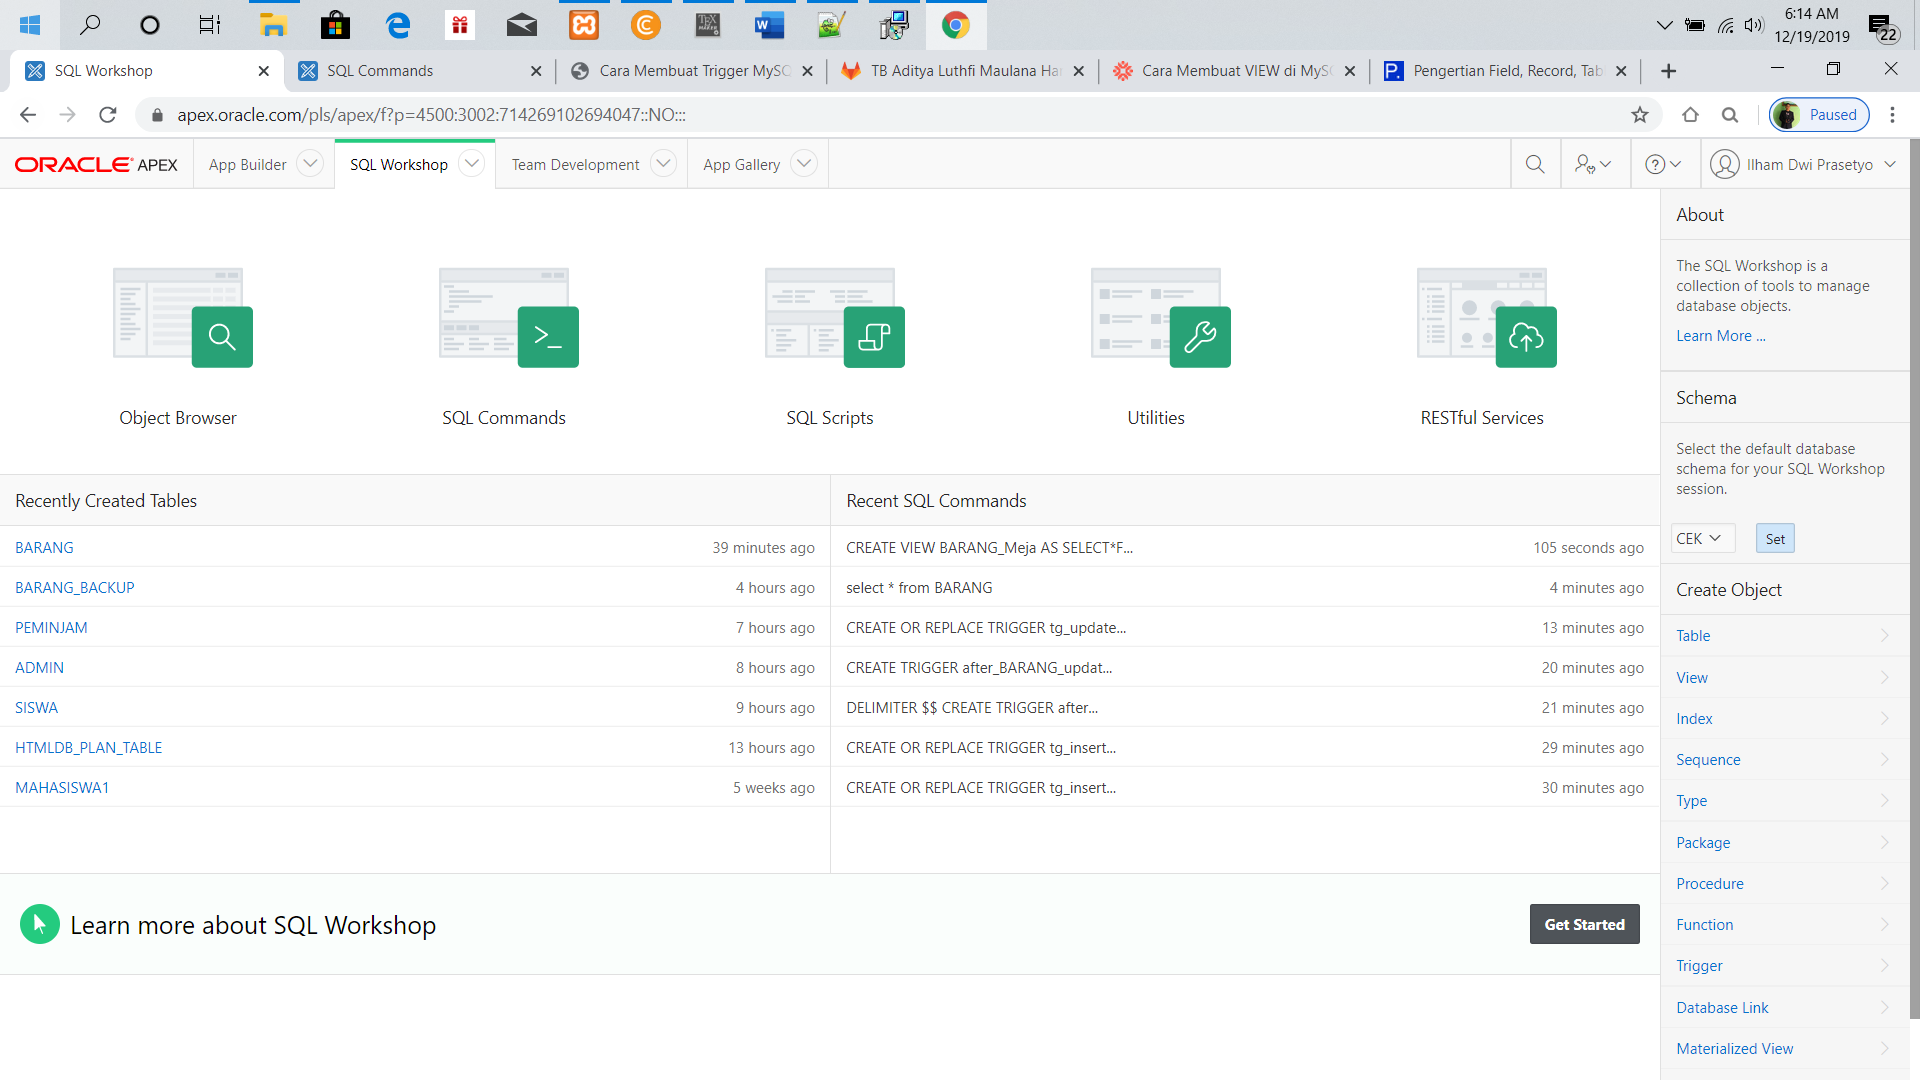
\includegraphics[scale=0.3]{img/2.PNG}
\end{figure}
\\
\\
\\
\\
\\
\\
\\
\
\
\
\
\par lalu klik sql command untuk pembuatan table
\begin{figure}[h]
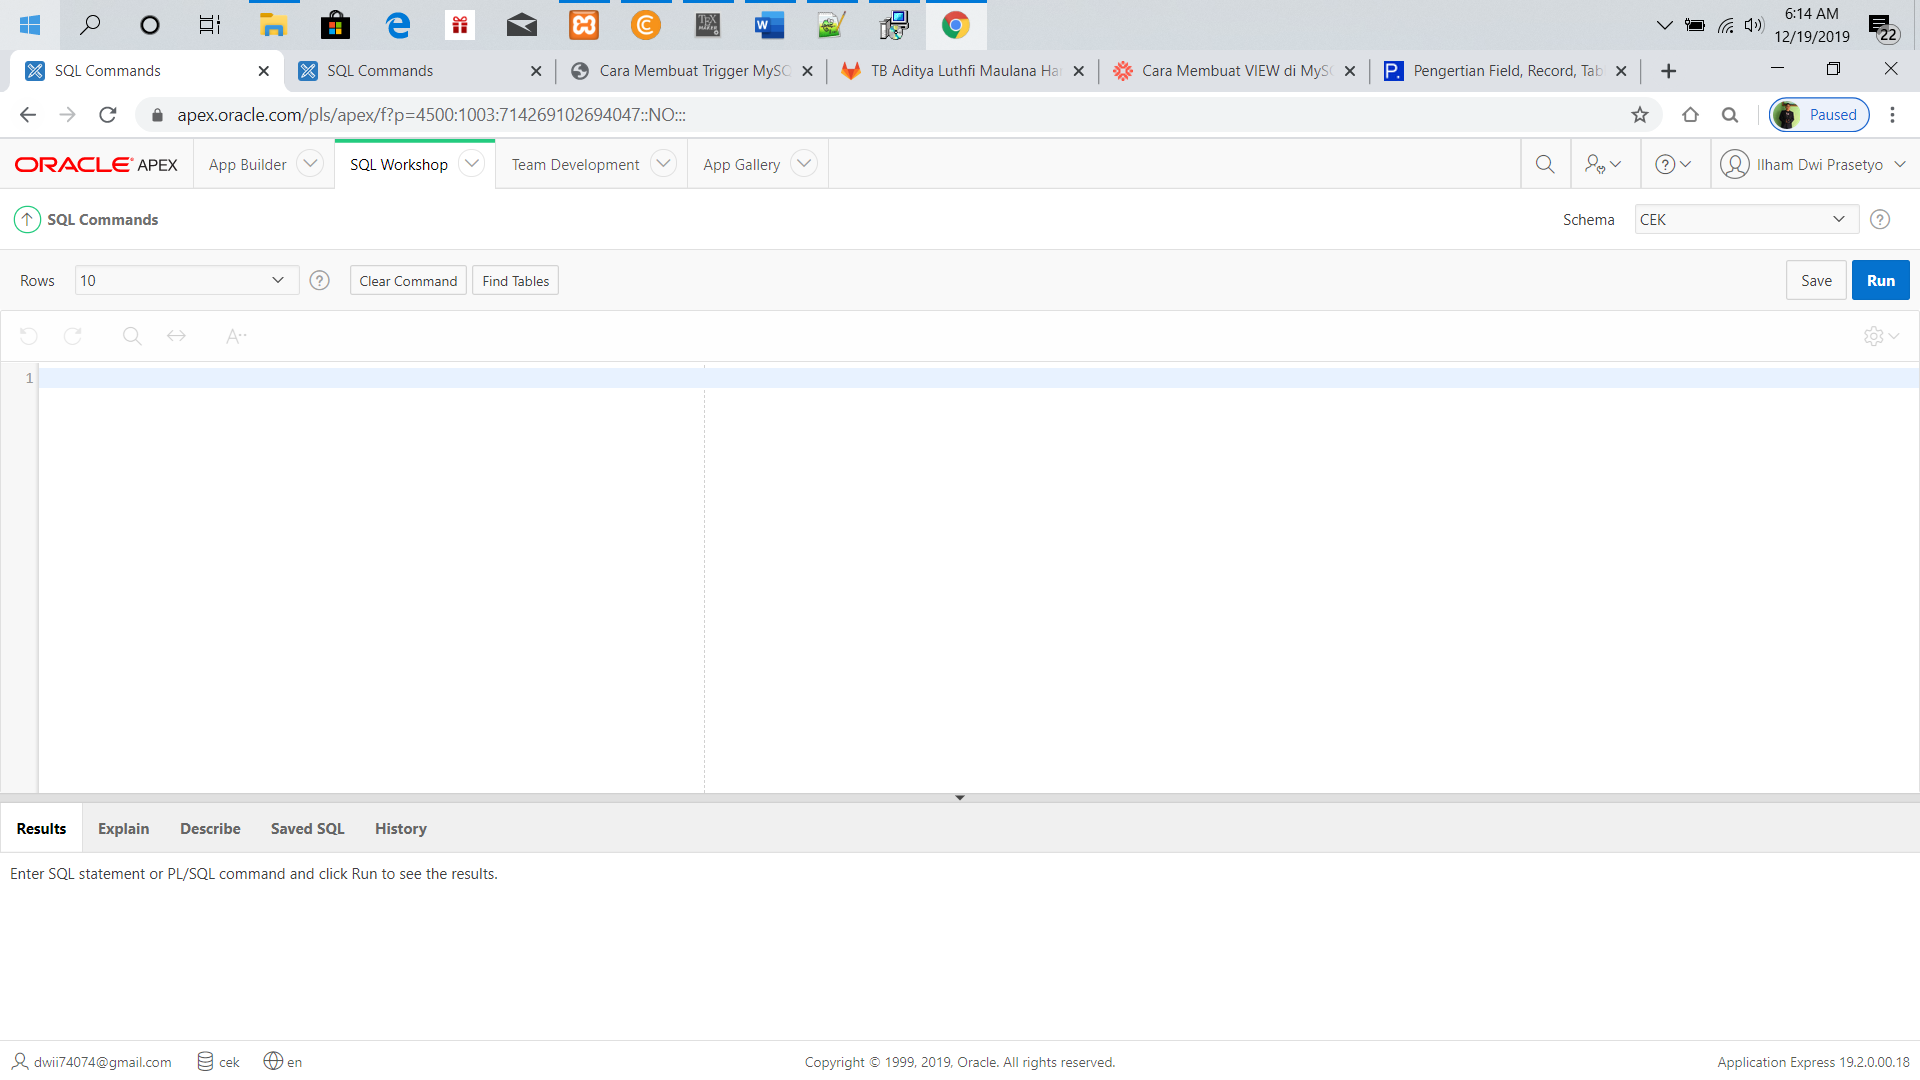
\includegraphics[scale=0.3]{img/3.PNG}
\end{figure}
\\
\\
\\
\\
\\
\\
\\
\\
\\
\\
\\
\\
\\
\par buatlah table barang di command dengan query sebagai berikut
\begin{figure}[h]
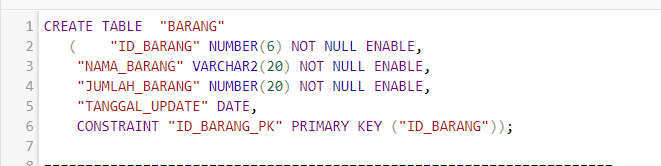
\includegraphics[scale=0.3]{img/4.PNG}
\end{figure}
\\
\\
\\
\\
\\
\\
\\
\\
\\
\\
\\
\\
\\
\par setelah selesai buatlah table barang backup
\begin{figure}[h]
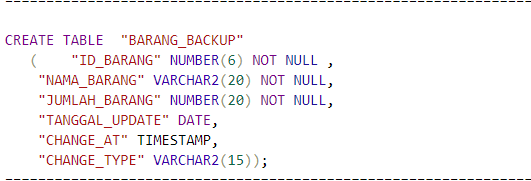
\includegraphics[scale=0.3]{img/5.PNG}
\end{figure}
\\
\\
\\
\\
\\
\\
\\
\\
\\
\\
\\
\\
\\
\\
\\
\par setelah membuat kedua table akan tampil sebagai berikut
\begin{figure}[h]
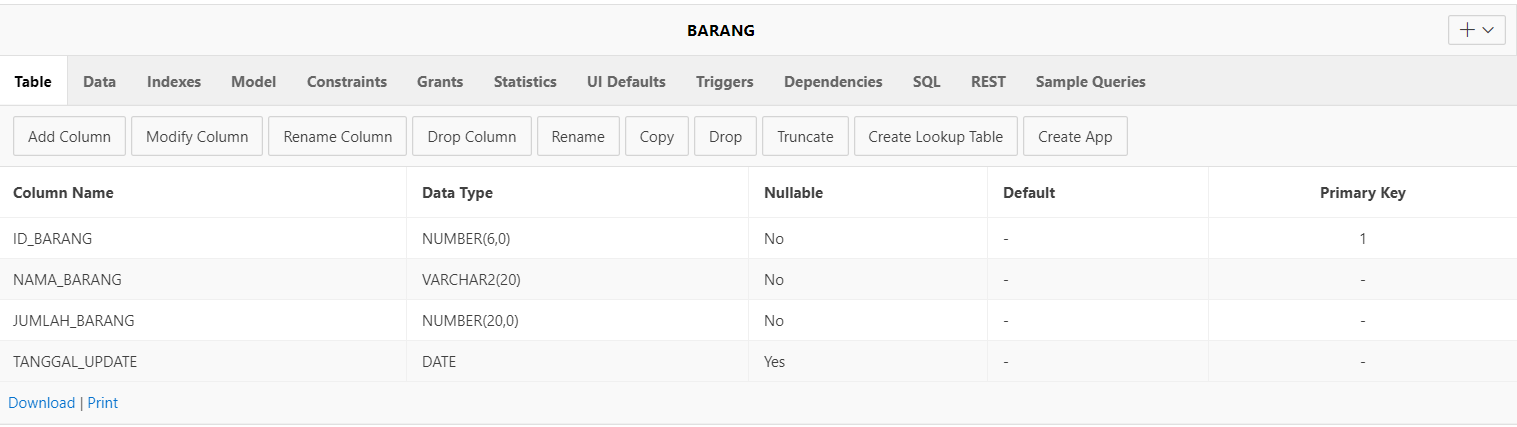
\includegraphics[scale=0.3]{img/9.PNG}
\end{figure}
\\
\\
\\
\\
\\
\\
\\
\\
\\
\\
\\
\begin{figure}[h]
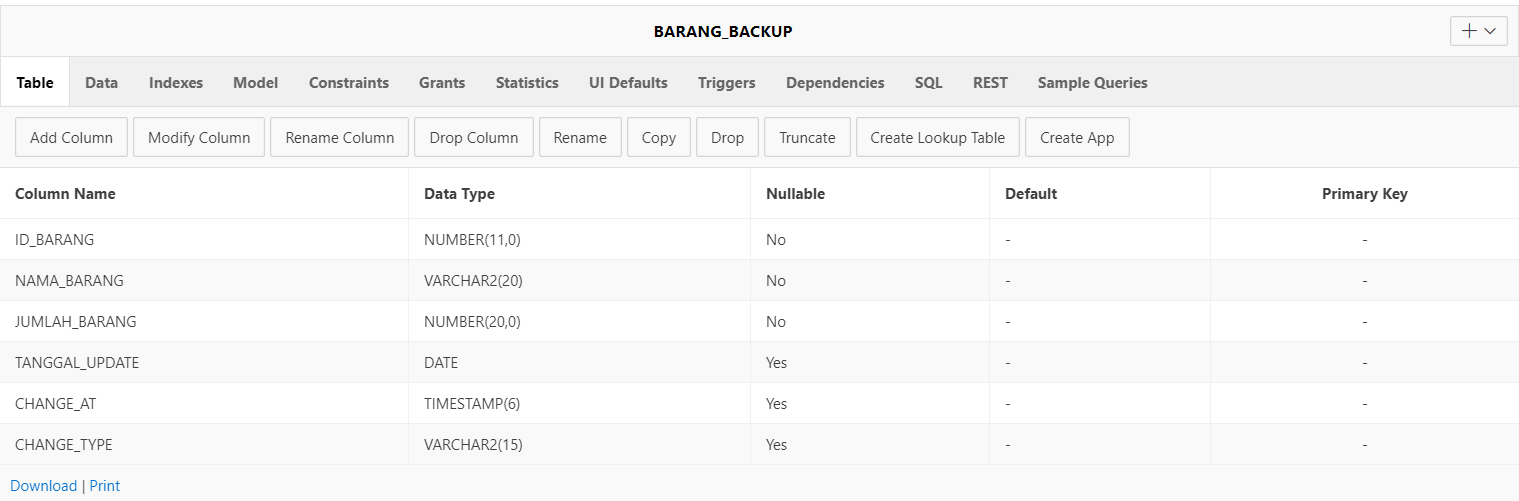
\includegraphics[scale=0.3]{img/10.PNG}
\end{figure}
\\
\\
\\
\\
\\
\\
\\
\\
\\
\\
\\
\\
\par setelah itu buat table admin danadmin back up dengan query berikut
\begin{figure}[h]
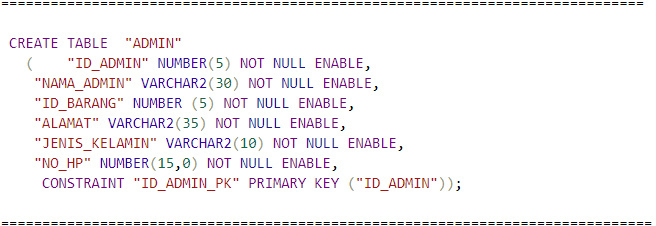
\includegraphics[scale=0.3]{img/11.PNG}
\end{figure}
\\
\\
\\
\\
\\
\\
\\
\\
\\
\\
\\
\\
\begin{figure}[h]
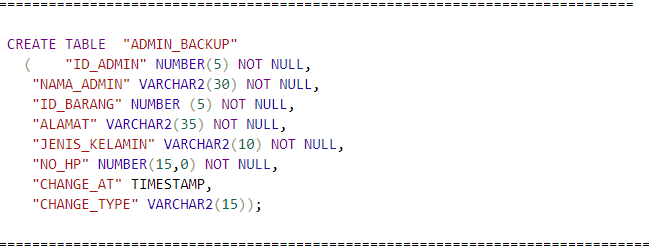
\includegraphics[scale=0.3]{img/12.PNG}
\end{figure}
\subsection{trigger}
\par query pembuata trigger update, insert, dan delete pada table barang sebagai berikut
\begin{figure}[h]
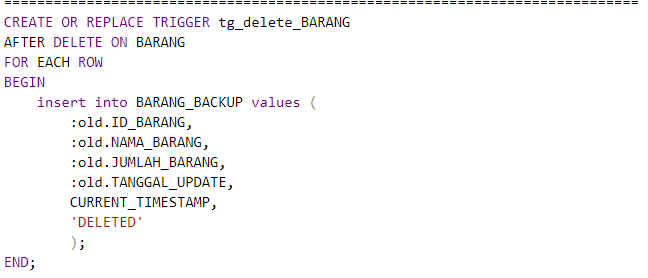
\includegraphics[scale=0.5]{img/6.PNG}
\end{figure}
\begin{figure}[h]
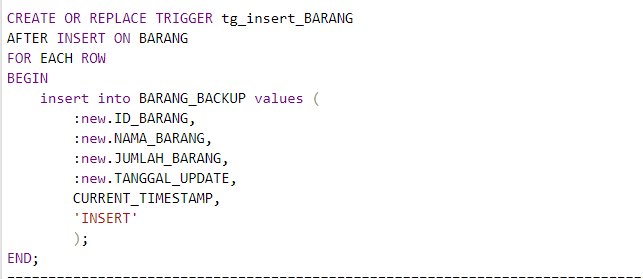
\includegraphics[scale=0.5]{img/7.PNG}
\end{figure}
\begin{figure}[h]
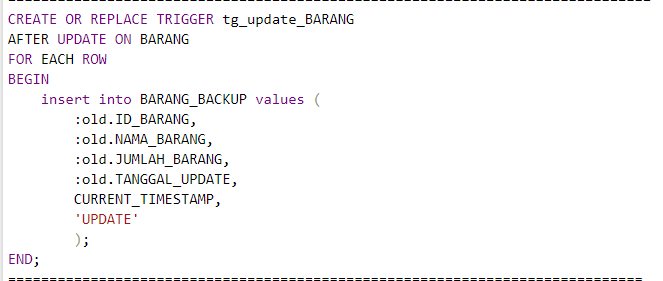
\includegraphics[scale=0.5]{img/8.PNG}
\end{figure}

\par query trigger update,insert,delete pada table admin sebagai berikut
\begin{figure}[h]
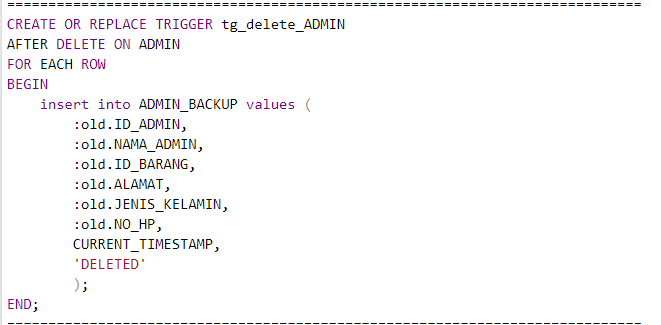
\includegraphics[scale=0.3]{img/13.PNG}
\end{figure}
\begin{figure}[h]
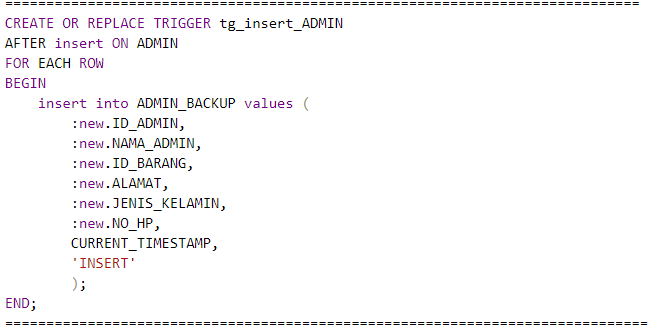
\includegraphics[scale=0.3]{img/14.PNG}
\end{figure}
\begin{figure}[h]
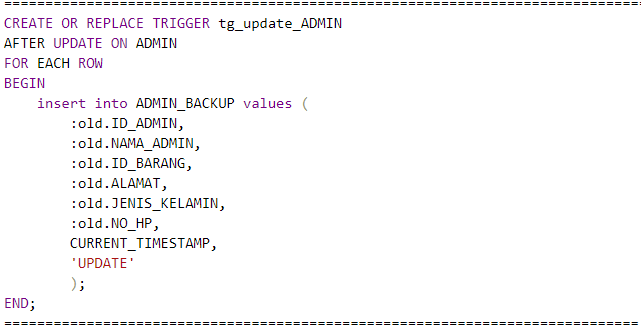
\includegraphics[scale=0.3]{img/15.PNG}
\end{figure}
\\
\\
\\
\\
\\
\\
\\
\\
\\
\\
\subsection{pembuatan aplikasi}
\par setelah semua telah selesai dibuat, langsung creat aplikasi dengan cara create aplikasi lalu masukkan data yang sudah di buat kemudain beri nama setelah itu beri nama apikasi yang kita akan buat lalu klik create dan akan tampil sebagai berikut
\begin{figure}[h]
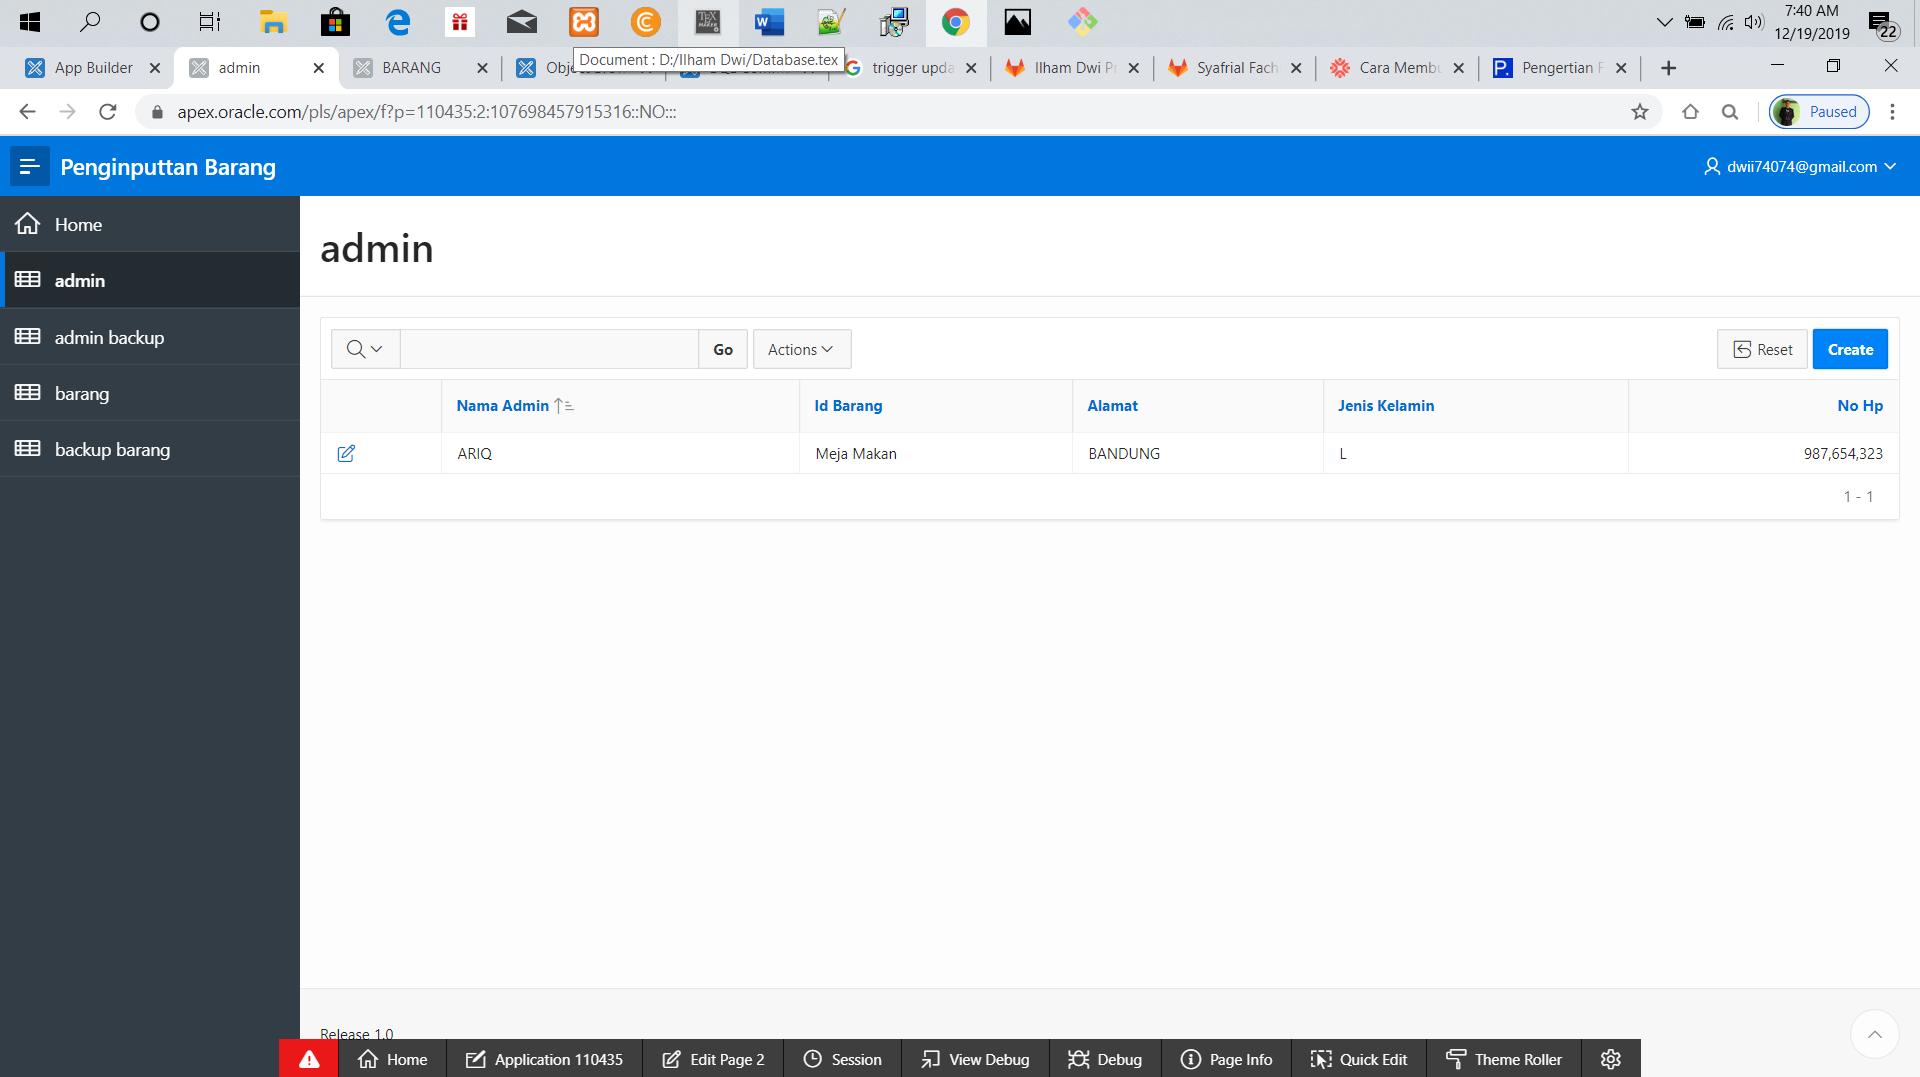
\includegraphics[scale=0.3]{img/16.PNG}
\end{figure}
\\
\\
\\
\\
\\
\\
\\
\\
\\
\\
\\
\\

\subsection{LINK}
\par LINK :
https://apex.oracle.com/pls/apex/f?p=4500:1000:705351505969591:::::

cek
Username :
dwii74074@gmail.com
password :
ilhamdwi170214
\end{document}
